\documentclass[a4paper,10pt]{article}
\usepackage[utf8]{inputenc}

\setlength\parindent{0pt}
\usepackage[english]{babel}
\usepackage[dvinames]{xcolor}
\usepackage[compact,small]{titlesec}
\usepackage{booktabs}
\usepackage{multirow}
\usepackage{amsfonts,amsmath,amssymb}
\usepackage{marginnote}
\usepackage[top=1.8cm, bottom=1.8cm, outer=1.8cm, inner=1.8cm, heightrounded, marginparwidth=2.5cm, marginparsep=0.5cm]{geometry}
\usepackage{enumitem}
\setlist{noitemsep,parsep=2pt}
\newcommand{\highlight}[1]{\textcolor{kuleuven}{#1}}
\usepackage{pythonhighlight}
\usepackage{cleveref}
\usepackage{graphicx}
\usepackage{algorithmic}
\usepackage{tabularx}

\newcommand{\nextyear}{\advance\year by 1 \the\year\advance\year by -1}
\newcommand{\thisyear}{\the\year}
\newcommand{\deadlineGroup}{November 27, \thisyear{} at 16:00 CET}
\newcommand{\deadlineCode}{December 18, \thisyear{} at 16:00 CET}
\newcommand{\deadlineReport}{January 4, \nextyear{} at 16:00 CET}

\newcommand{\ReplaceMe}[1]{{\color{blue}#1}}
\newcommand{\RemoveMe}[1]{{\color{purple}#1}}

\setlength{\parskip}{5pt}

%opening
\title{Artificial Neural Networks: Exercise session 2}
\author{Stijn Staring (r0620003)}

\begin{document}
\fontfamily{ppl}
\selectfont{}

\maketitle


\section{Exercises of Section 1: Hopfield Network}
\textbf{Create a Hopfield network with attractors T = [1 1;-1  -1; 1 -1]T and the corresponding number of neurons. You
	can use script rep2 as a basis and modify it to start from some particular points (e.g. of high symmetry) or to generate
	other numbers of points. Start with various initial vectors and note down the obtained attractors after a sufficient number
	of iterations. Are the real attractors the same as those used to create the network? If not, why do we get these unwanted
	attractors? How many iterations does it typically take to reach the attractor? What can you say about the stability of the
	attractors?}\\

In Figure \ref{fig:rep2Attractors} all the found attractors can be seen which are more than the three desired ones that were specified to the Hopfield network. It can thus concluded that the despite the ``newhop'' matlab function tries to design a Hopfield network with the minimum of unspecified target attractors, they often occur. Table \ref{tab:attractors} shows the found attractor points. when designing the energy function for the system that has a corresponding local minima on at the attractor points, it can be that also unwanted attractor points become local minima. When the assumption of no bais term of the model is made, these correspond with the negative of the desired attractors. Also, a mixture of the desired states are possible. The amount of iterations it takes to reach an attractor depends on the start position. All the symmetric starting points of Figure \ref{fig:rep2Attractors} reached an atractor in less then $ 5 $ iterations. However, the amount of iterations can dramatically increase when the starting point is very close to an unstable attractor. For example when the starting point chosen is: $ [-1;-10^{-20}] $ it takes $ 308 $ iteration to reach the stable attractor $ [-1;-1] $. When the system is in a stable attractor and a little noise is added the system will move back to the stable attraction point. An unstable attractor on the other hand will move away when this happens. The stability of the diffent attractor points can be seen in Table \ref{tab:att}.


\begin{figure}[h!]
	\centering
	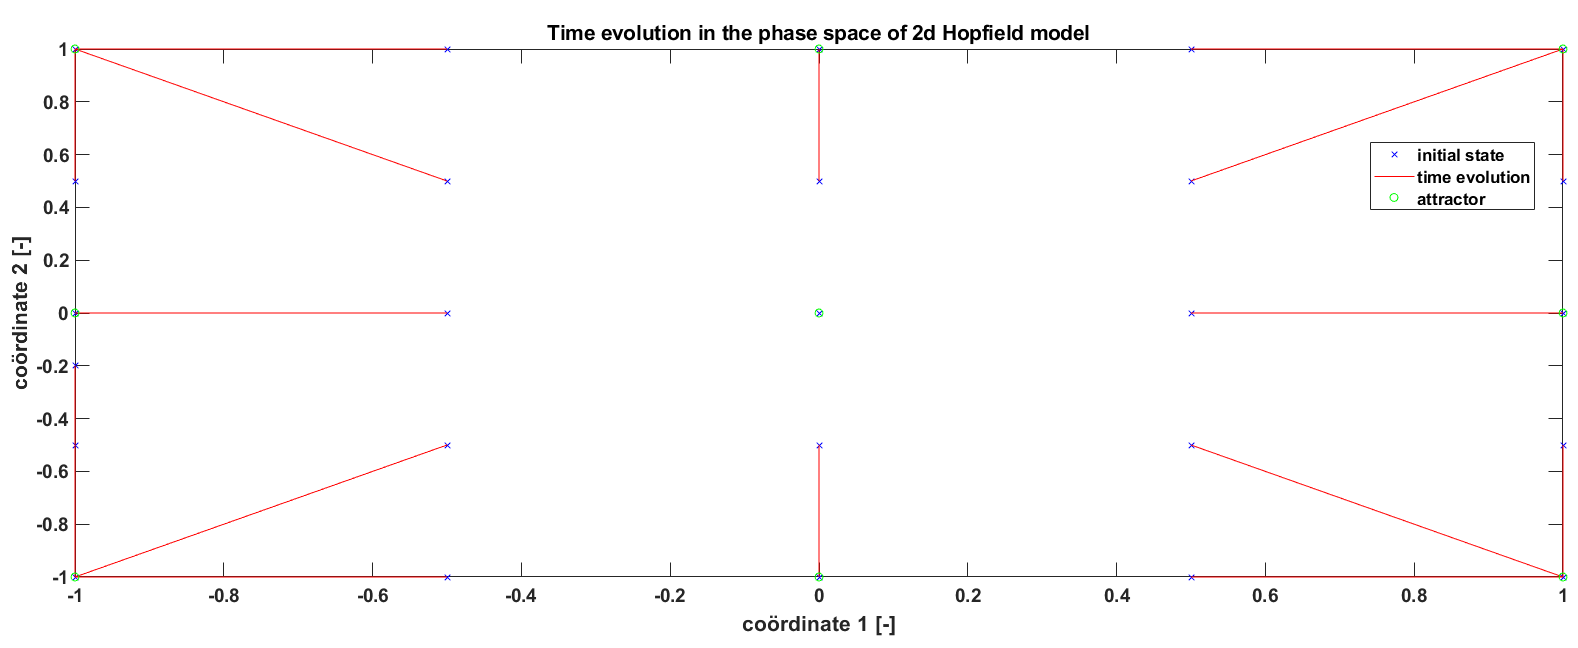
\includegraphics[width=1.\textwidth]{rep2Attractors.png}
	\caption{All the found attractors.}
	\label{fig:rep2Attractors}
\end{figure}


\begin{table}
	\centering
	\begin{tabular}{@{}clr@{}} \toprule
		\textbf{Attractor} & \textbf{Point} & \textbf{Stability}\\\midrule
		Attractor $ 1 $ & $ [1;1] $ & Stable\\
		Attractor $ 2 $ & $ [-1;-1] $ & Stable\\
		Attractor $ 3 $ & $ [1;-1] $ & Stable\\
		Attractor $ 4 $ & $ [-1;1] $ & Stable\\
		Attractor $ 5 $ & $ [0;0] $ & Unstable\\
		Attractor $ 6 $ & $ [0;1] $ & Unstable\\
		Attractor $ 7 $ & $ [0;-1] $ & Unstable\\
		Attractor $ 8 $ & $ [1;0] $ & Unstable\\
		Attractor $ 9 $ & $ [-1;0] $ & Unstable\\\bottomrule
	\end{tabular}
	\caption{Overview of the different attractor points found in a 2D plane.}
	\label{tab:att}
\end{table}

Table \ref{tab:att3} shows an overview of the found attractors in a 3D space. Only the three specified target attractors were found during the experimentation with different starting points. All three are stabel points. 
\begin{table}
	\centering
	\begin{tabular}{@{}clr@{}} \toprule
		\textbf{Attractor} & \textbf{Point} & \textbf{Stability}\\\midrule
		Attractor $ 1 $ & $ [1;1;1] $ & Stable\\
		Attractor $ 2 $ & $ [-1;-1;1] $ & Stable\\
		Attractor $ 3 $ & $ [1;-1;-1] $ & Stable\\\bottomrule
	\end{tabular}
	\caption{Overview of the different attractor points found in a 3D plane.}
	\label{tab:att3}
\end{table}
\newpage
\textbf{The function hopdigit creates a Hopfield network which has as attractors the handwritten digits 0,...,9. Then to test
	the ability of the network to correctly retrieve these patterns some noisy digits are given to the network. Is the Hopfield
	model always able to reconstruct the noisy digits? If not why? What is the influence of the noise on the number of
	iterations?}\\

The noise that is added to the digits is gaussian noise. The noise variable determines the standard deviation of the gaussian that is sampled from to retrieve the noise that should be added. It can be concluded that when the noise is too high, the Hopfield model is not able to reconstruct the correct digits. The reason is because when the noise is too heavy the starting point can become closer to other digits than the original one. Increasing the amount of iterations will not solve this issue. When there is more noise, the system needs more iterations to reach the attractor points.

\section{Exercises of Section 2: Long Short-Term Memory Networks}
\textbf{Train a MLP with one hidden layer after standardizing the data set. Investigate the model
performance with different lags and number of neurons. Explain clearly how do you tune the parameters and what is the influence on the final prediction. Which combination of parameters gives the best performance on the test set?}\\

In this section the time serie  signal included in the Santa Fe dataset will be forecasted. A training set of $ 1000 $ samples and a test set of $ 100 $ samples are given. The first step is to standardize the training data by subtracting the mean of the full time serie and dividing it afterwards by the standard deviation. This has as effect that the time serie is shifted to oscillate around data with a standard deviation of $ 1 $. The effect of standardization is in general that it speeds up the learning process during training. \\
The neural network consists out of a single hidden layer which uses as activation function ``tanh''. The amount of input neurons is dependent on the lag value. The lag value determines how many past samples of the time-serie are taken into account to make the forecast. There is only one output neuron that gets inputs from all the hidden neurons and uses the ``purelin'' activation function. One time-serie sample is predicted at the time and therefore to make a prediction of a longer time horizon, multiple predictions have to be sequentially performed using previous ones as inputs of the next.\\

A parameter search is conducted to determine the amount of neurons in the hidden layer, the lag value and the regulation parameter. The regulation parameter determines the importance of the $ L2 $ norm in the objective function. As update rule the ``Gradient descent'' method is used. Table \ref{tab:design} gives an overview of the different designs that were tested. $ 10\% $ of the training set is assigned to the validation set to perform early stopping to avoid overfitting.\\

\begin{table}
	\centering
	\begin{tabular}{@{}lr@{}} \toprule
		\textbf{Design Variable}    & Domain \\\midrule
		Regulation parameter & $ 0:0.2:0.4 $ \\ 
		Amount of hidden layers & $ 1 $\\
		Amount of neurons in hidden layer & $ 1:2:9 $  \\
		Learning rule & Gradient descent\\
		Training time per training session & $ 5 s $\\
		Max amount of sequential increases of the validation error in early stopping & $ 15 $\\
		Goal of training error & $ 10^{-3} $\\
		Amount of iterations to take average & $ 5 $\\\bottomrule
	\end{tabular}
	\caption{The different design variable and their corresponding domain.}
	\label{tab:design}
\end{table}  

It was found that the best results were obtained when when using a regulation parameter of $ 0.4 $, $ 9 $ hidden neurons and a lag value of $ 16 $ are used. The lowest MSE value retrieved is $ 2.94\times10^{-1} $. The MSE value is calculated as the average of $ 5 $ neural networks simulations that were trained with the same settings according to Table \ref{tab:design}, but with different randomly initialised weights. The error is the difference between the target values and the predicted values that were retrieved by sequentially predicting the next value while using previous predictions as new inputs. The selected design of the neural network is now used to learn for $ 5 $ minutes on the training data. This network is afterwards used to do predictions on the $ 100 $ samples of the test set which can be seen in Figure \ref{fig:After_simulation_of_5min_per}. It can be seen that in the beginning the first three peaks can be reasonably approximated but the error increases rapidly when the predictions are further in time due to a cumulative error effect. However this is not the only reason for the bad behaviour of the forecast after sample $ 50 $. A test is performed where a forecast starts from sample $ 50 $ which is just at the moment that the test set shows a reset of the magnitude of the oscillation. It can be seen that the neural network gives still unsatisfactory results because it can not identify the ``reset'' but predicts big peaks instead. The MSE value of the prediction displayed in Figure \ref{fig:After_simulation_of_5min_per} is $ 2.54\times10^{3} $.

\begin{figure}[h!]
	\centering
	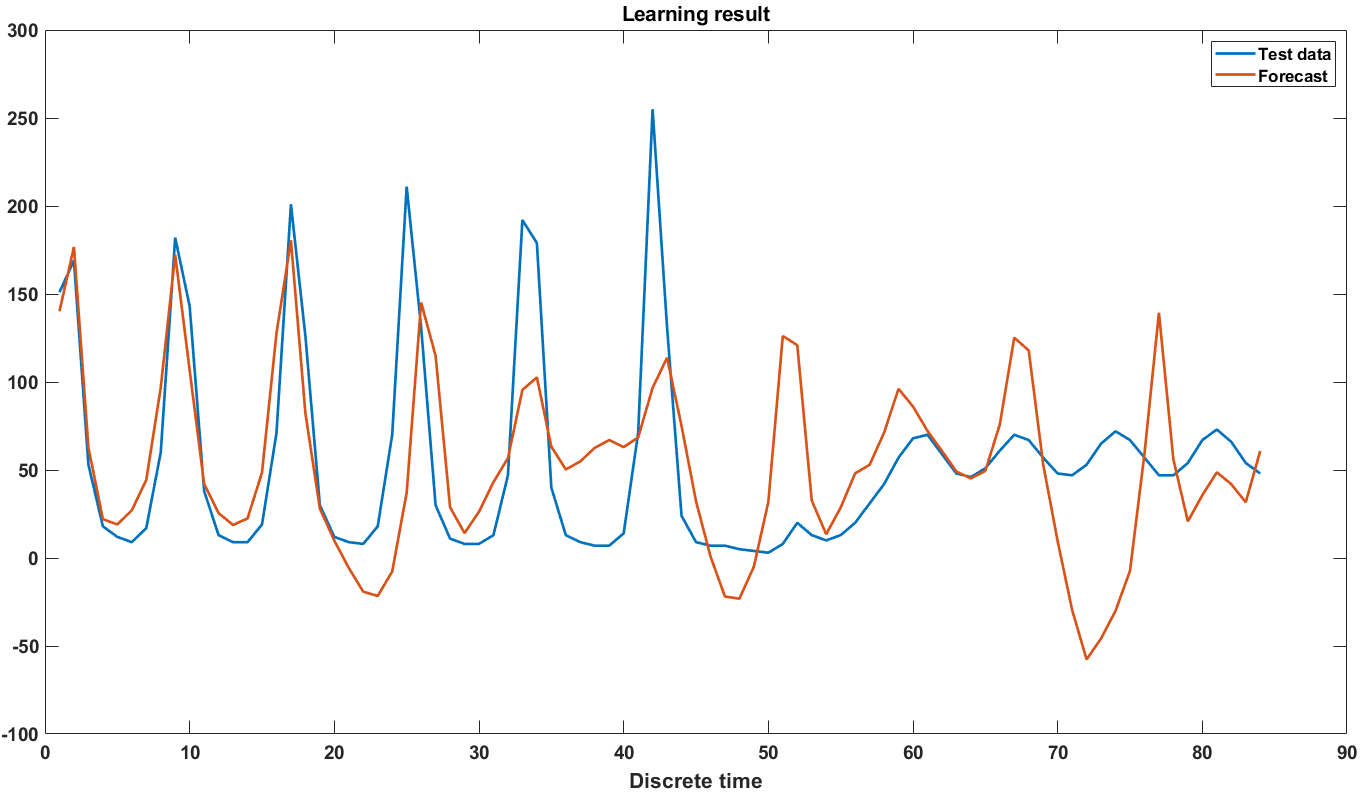
\includegraphics[width=0.8\textwidth]{learning_result.png}
	\caption{The forecasting result on the test set with the selected Neural Network that is trained for $ 5 $ minutes.}
	\label{fig:After_simulation_of_5min_per}
\end{figure}

\textbf{Implementation of LSTM}\\
Next, a LSTM (long short term memory) neural network will be assessed to model the Santa Fe data set instead of the MLP regression neural network that was used in the previous section . A LSTM has as advantage over a standard RNN that I can better handle the vanishing gradient problem and LSTM is not suffering as much of a short term memory. Therefore, it can  longer take important aspects of the presented time-serie into account when working on a new forecasting. LSTM makes use of three gates to learn which data of the sequence is important and should be remembered. In connection of these gates is a cell state which serves as a memory state and a connection to transport relative information throughout the different time steps. The forget gate decides what information should be kept or removed from the input and hidden state. The input gate updates the cell state and the output state decides what the next hidden state will be.\\
In order to train a LSTM neural network there are more parameters that have to be learned.  There are now four different weight matrices. One form the forget gate, two from the input gate and one from the output gate. It can be noted that in order to train all these weights, this network is more data hungry than a simple RNN. 




\begin{itemize}
	\item Stijn
\end{itemize}

















%\cite{fast_alg}
%\cite{inver_over}

\bibliographystyle{abbrv}
%\bibliography{ANN1}

\end{document}
